\section{Topic}
	\subsection{Brief Task Description}
	This project is about implementing the game Pong on the Atlys Spartan-6 FPGA board. Pong is a two dimensional multiplayer game that simulates table-tennis. Each of the two players controls an in game paddle by moving it vertically in order to hit a ball back and forth. A player scores a point when the opponent fails to return the ball. 
	
	We also took advantage of the built-in HDMI port and the AC-97 Codec to produce a better image and audio quality output. 
	
	Figure \ref{board+screenshot} shows a picture of the used board, and a screenshot of the \textcolor{red}{(yet to be)} realized game. 
	
	\begin{figure}[h]
		\begin{subfigure}[b]{.4\textwidth}
			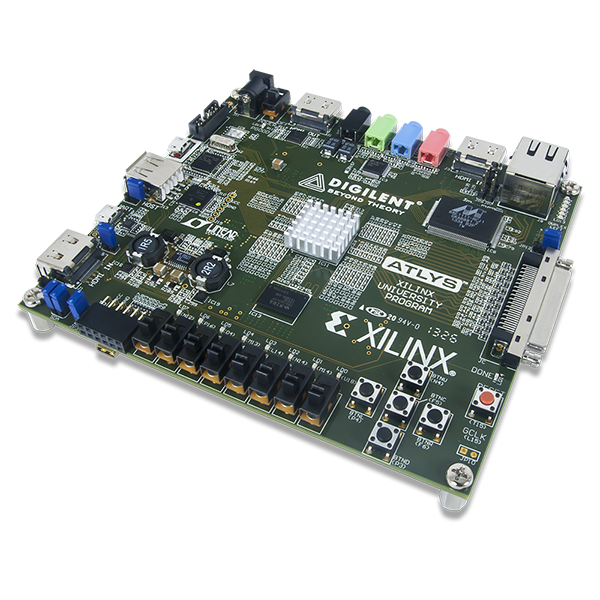
\includegraphics[width=8cm]{images/atlys_pic.png}
			\caption{Atlys Spartan-6 board}
		\end{subfigure}
		\hfill
		\begin{subfigure}[b]{.4\textwidth}
			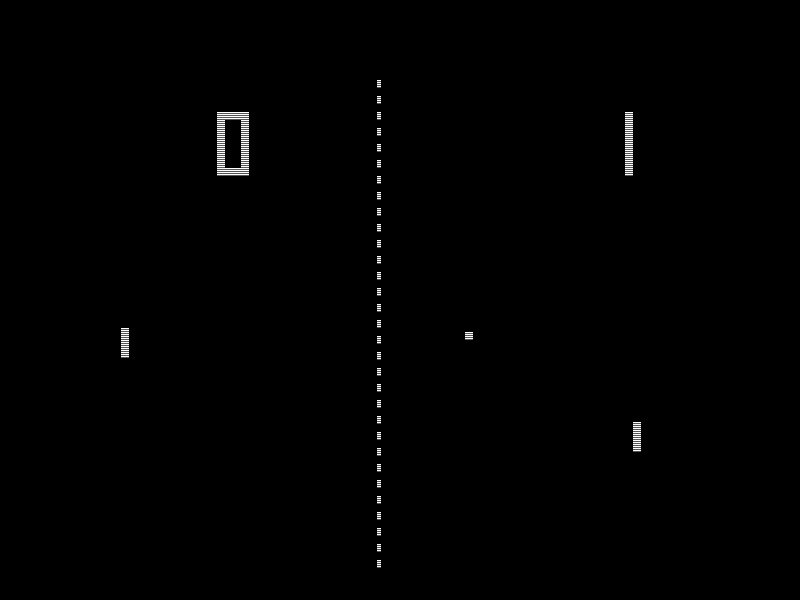
\includegraphics[width=8cm]{images/pong_screenshot.png}		
			\caption{Screenshot of the game Pong}
		\end{subfigure}
		
	\caption{Used board and screenshot of the game}
	\label{board+screenshot}
	\end{figure}
	
	
	\subsection{Block Diagrams}
		Figure \ref{img_gen} shows the block diagram of the module \texttt{image\_generator\_c}. Figure \ref{snd_gen} show
		
	\begin{figure}[here]
		\centering
		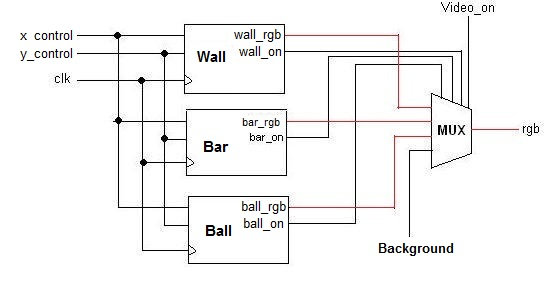
\includegraphics[scale=0.7]{images/img_gen.jpg}
		\caption{Schematic of the Image Generator}
		\label{img_gen}
	\end{figure}
	
	\begin{figure}[here]
		\centering
		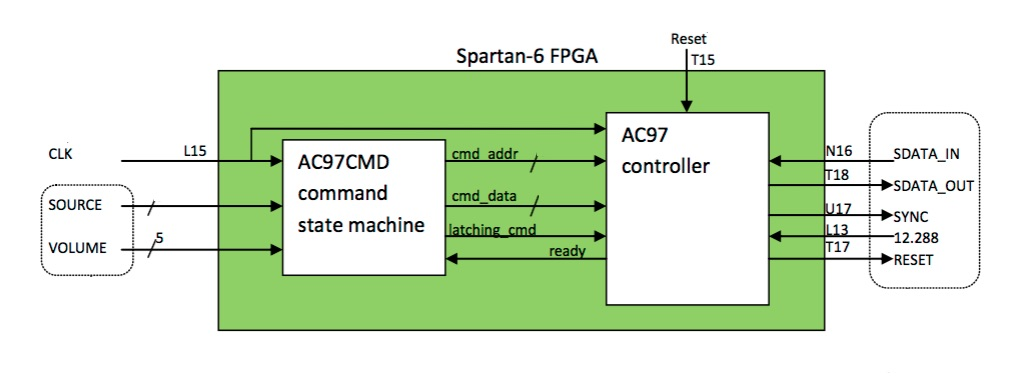
\includegraphics[scale=0.5]{images/snd_gen.jpg}
		\caption{Block diagram of the Sound Generator}
		\label{snd_gen}
	\end{figure}
	
	
	
	%\begin{figure}[here]
%		\centering
%		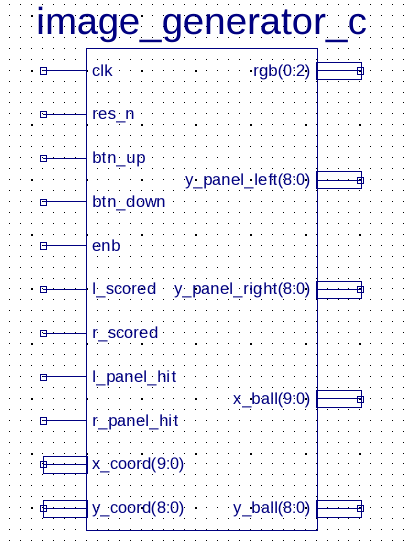
\includegraphics[scale=0.35]{images/image_generator_c.png}
%		\caption{Schematic of Image Generator}
%		\label{image_generator}
%	\end{figure}
		
	%\begin{figure}[h]
%		\centering
%		\begin{subfigure}[b]{.4\textwidth}
%			\centering
%			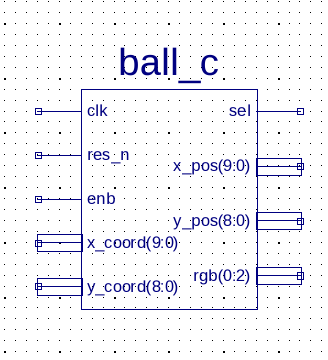
\includegraphics[scale=0.35]{images/ball_c.png}
%			\caption{Schematic of the in-game ball}
%		\end{subfigure}
%		\hfill
%		\begin{subfigure}[b]{.4\textwidth}
%			\centering
%			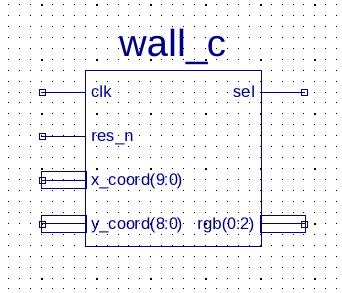
\includegraphics[scale=0.35]{images/wall_c.png}		
%			\caption{Schematic of the in-game wall}
%		\end{subfigure}
%		\hfill
%		\begin{subfigure}[b]{.4\textwidth}
%			\centering
%			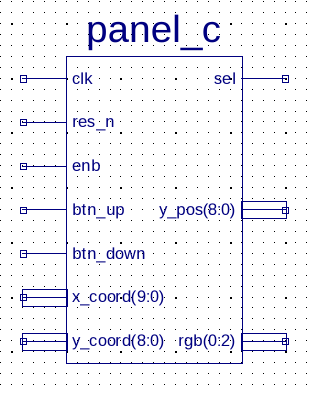
\includegraphics[scale=0.35]{images/panel_c.png}		
%			\caption{Schematic of the in-game panel}
%		\end{subfigure}
		
%	\caption{Schematics of the sub-modules of the image generator module}
%	\label{ball_wall_panel}
%	\end{figure}

	\newpage	
	\subsection{Functional Details}
		\subsubsection{Image Generator}
		The Image Generator takes inputs from the players and outputs the video that can be displayed through the HDMI interface of the Atlys board. The panels shown in figure \ref{ball_wall_panel} are submodules of the module \texttt{image\_generator\_c}.
		This module calculates the movement of the ball and movement the two panels that are controlled by the players. 
		
		The movement of the ball is done by the \texttt{ball\_c} module. (see next Section for more details on implementation).
		After a well determined time frame, the ball's movement direction is determined and the next \texttt{x\_pos} and \texttt{y\_pos} are either incremented or decremented. 
		
		The module \texttt{panel\_c} determines the y-coordinate of on panel based on the player input. For instance, pressing \texttt{btn\_up} increments the \texttt{y\_pos} signal if the panel did not reach the top edge already. 


		  \subsubsection{Sound Generator}
				In order to generate sound, we used the on board LM4550 chip
		  
\newpage
	
